\titre{}
\theme{derivation}
\auteur{Nathan Scheinmann}
\niveau{3M}
\source{sesamath3e}
\type{serie}
\piments{2}
\pts{}
\annee{2425}

\contenu{
\tcblower
Sur le graphique ci-dessous on a représenté une fonction \(g\) pour \(x\in[-4;5{,}5]\) :
% (graphique)
	\begin{center}
		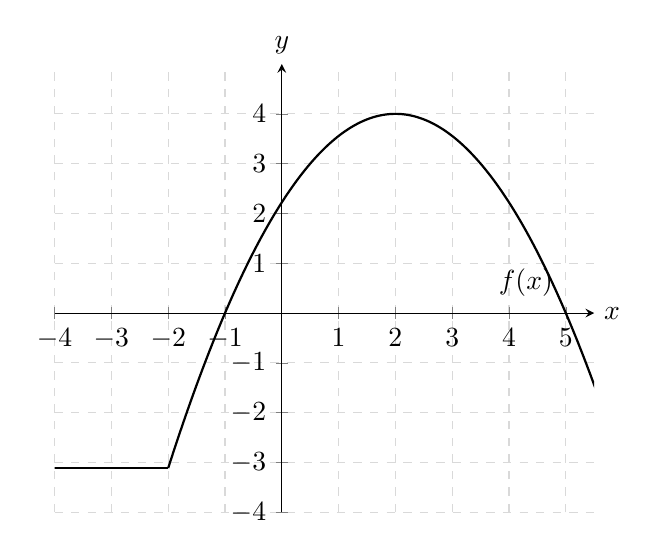
\begin{tikzpicture}
  \begin{axis}[
    axis lines=middle,
    xlabel={$x$}, ylabel={$y$},
    xlabel style={at=(current axis.right of origin), anchor=west},
    ylabel style={at=(current axis.above origin), anchor=south},
    xmin=-4, xmax=5.5, ymin=-4, ymax=5,
    xtick={-4,-3,-2,-1,0,1,2,3,4,5},
    ytick={-4,-3,-2,-1,0,1,2,3,4},
    grid=both,
    grid style={dashed,gray!30},
  ]
    % branche pour x < -1
    \addplot [domain=-5:-2, samples=200, thick]
      {-4/9*(-2+1)*(-2-5)};
    \addplot [domain=-2:6, samples=200, thick]
      {-4/9*(x+1)*(x-5)} node[above left,pos=0.8] {$f(x)$};
  \end{axis}
\end{tikzpicture}
	\end{center}
\begin{tasks}(1)
  \task Esquisser aussi précisément que possible la représentation graphique de la fonction dérivée \(g'\).
  \task Sur le même repère, mais avec une autre couleur, tracer une courbe \(h\) qui passe par le point \(P(0;-2)\) et telle que \(h'(x)=g(x)\).
\end{tasks}
}
\correction{
\tcblower
\textit{Generated by AI}

D'après le graphique, la fonction $g(x) = -\frac{4}{9}(x+1)(x-5)$ est une parabole.

\begin{tasks}(1)
\task \textbf{Esquisser la dérivée $g'$ :}

Développons d'abord $g$ :
\[g(x) = -\frac{4}{9}(x^2 - 4x - 5) = -\frac{4}{9}x^2 + \frac{16}{9}x + \frac{20}{9}\]

Donc :
\[g'(x) = -\frac{8}{9}x + \frac{16}{9} = \frac{8}{9}(2 - x)\]

La dérivée $g'$ est une fonction affine (droite) :
\begin{itemize}
\item $g'(x) = 0$ quand $x = 2$ (la parabole a son sommet en $x=2$)
\item $g'(x) > 0$ pour $x < 2$ (fonction croissante)
\item $g'(x) < 0$ pour $x > 2$ (fonction décroissante)
\item C'est une droite décroissante qui passe par $(2, 0)$
\end{itemize}

\task \textbf{Tracer $h$ telle que $h'(x) = g(x)$ et passant par $P(0, -2)$ :}

Si $h'(x) = g(x) = -\frac{4}{9}x^2 + \frac{16}{9}x + \frac{20}{9}$, alors $h$ est la primitive de $g$ :

\[h(x) = -\frac{4}{27}x^3 + \frac{8}{9}x^2 + \frac{20}{9}x + C\]

Pour trouver $C$, utilisons $h(0) = -2$ :
\[h(0) = C = -2\]

Donc :
\[h(x) = -\frac{4}{27}x^3 + \frac{8}{9}x^2 + \frac{20}{9}x - 2\]

Cette fonction est cubique, croissante où $g > 0$ et décroissante où $g < 0$.
\end{tasks}
}

